\chapter{Métricas de código-fonte}
\label{cap-metrics-esw} 


Tanto a existência de um bom \emph{design} quanto a de testes automatizados que exercitem as funcionalidades são características desejáveis em projetos de software. Boa parte das técnicas modernas da Engenharia de Software são voltadas para desenvolvimento com design que proporcione simplicidade, manutenibilidade e testabilidade. Mesmo que a maior parte dessas técnicas tenham sido disseminadas a partir do advento dos Métodos Ágeis e do Software Livre, cujo foco central está em atividades relacionadas ao código-fonte, elas são aplicáveis independentemente da metodologia de desenvolvimento utilizada \cite{meirelles2013metrics}. A valorização por softwares que atendam esses parâmetros de qualidade deve-se ao fato de sempre que o Engenheiro de Software está escrevendo novas linhas de código, um tempo significativo é gasto por ele na leitura e entendimento do código existente, muitas vezes desenvolvidos por outros Engenheiros. Martin (\citeyear{martin2008}) destaca que o código-fonte deve ser escrito para ser entendido principalmente por pessoas, e não pela máquina.

%

Nesse sentido, o monitoramento da qualidade de código-fonte pode ser utilizado para apoiar a utilização de técnicas de desenvolvimento que visam a melhoria contínua do código. Além disso, as métricas de código-fonte são muito importantes para projetos de software, pois estas podem ser utilizadas tanto como ferramenta para gestão do projeto quanto como referência técnica para tomada de decisões sobre o código-fonte.

%

Uma métrica, no âmbito da Engenharia de Software, provê uma forma de medir quantitativamente atributos relacionados as entidades do software e do processo de desenvolvimento. Assim, métricas são importantes ferramentas para avaliação da qualidade do código-fonte produzido e acompanhamento do projeto. Meirelles (\citeyear{meirelles2013metrics}) destaca que, com métricas de software, propõe-se uma melhoria de processo de gestão com identificação, medição e controle dos parâmetros essenciais do software.

%

Métricas de monitoramento de código-fonte possuem natureza objetiva e foram inicialmente concebidas para medir o tamanho e a complexidade do software \cite{henry1984kafura}\cite{troy1981zweben}\cite{yau1985zweben}. Outras métricas surgiram para avaliar softwares que utilizam paradigmas específicos, não sendo aplicáveis a qualquer tipo de software. Por exemplo, métricas Orientada a Objetos (OO) são usadas para avaliar sistemas orientados a objetos \cite{systa2000}. Métricas OO são destinadas, portanto, para avaliar a coesão de classes, as hierarquias de classes existentes, nível de acoplamento entre classes, reuso de código, dentre outras características.

%

Algumas características importantes ajudam a classificar as métricas de código-fonte. Assim, podemos classificá-las como estáticas e dinâmicas. Como o próprio nome diz, métricas estáticas capturam propriedades estáticas dos componentes de software e não necessita que o software seja executado para que seus valores sejam coletados. Por outro lado, métricas dinâmicas refletem características chaves tais como dependência dinâmica entre os componentes em tempo de execução do software.

%

No contexto desta monografia estamos interessados principalmente na análise estática de códigos-fontes. Nesse sentido, a análise estática é definida como o processo de avaliar um sistema ou seus componentes baseados em suas formas, estruturas, conteúdo ou documentação que podem gerar insumos para compreensão da qualidade de \emph{design} do código assim como enderaçar suas principais vulnerabilidades, podendo ser realizada sobre módulos e até mesmo sobre códigos ainda não finalizados \cite{black2009}. Esta análise pode ser realizada manualmente, tal como é feita em inspeções de código e com \emph{pair programming} ou de maneira automatizada através de ferramentas desenvolvidas para tal fim.

%

As métricas de software também podem ser classificadas quanto ao método de obtenção. Métricas primitivas podem ser diretamente coletadas refletindo um valor observável de um atributo, sendo raramente interpretadas independentemente. Por outro lado, métricas compostas são obtidas a partir da relação de uma ou mais métricas, derivada, por exemplo, a partir de uma expressão matemática.

%

Entretanto, as definições de métricas adequadas para o acompanhamento do projeto, dimensionamento do software e principalmente para a aferimento da qualidade do código-fonte são tarefas que aumentam a complexidade de adoção de métricas em projetos de software, assim como destacado por Rakić e Budimac (\citeyear{rakic2011budimac}).
%
Isso se deve a diversos fatores: à grande quantidade de métrica existentes; pouca aderência de algumas métricas com a realidade; diversas formas de interpretação de dados; dificuldades de definir parâmetros para comparação; poucos recursos de visualização de dados; coleta de dados não automatizados ou difíceis.
%
Fenton e Pfleeger (\citeyear{fenton1998}) definem características desejáveis de métricas que orientam a escolha das mesmas enquanto outros autores estudam formas de viabilizar a utilização de métricas pelos desenvolvedores em geral\cite{meirelles2013metrics,almeida2010}.
%
O presente trabalho visa relacionar métricas de desenvolvimento de software com objetivo de definir configurações para estabelecer cenários que representem o estado da qualidade do software. Dessa forma, espera-se reduzir as dificuldades de utilização de métricas de código fonte, tanto para o acompanhamento gerencial quanto para a tomada de decisões de \emph{design} por desenvolvedores baseada em evidências. Para tanto, nas próximas seções serão apresentados estudos realizados sobre métricas de monitoramento de código-fonte para sistemas orientados à objetos e métricas para avaliação de vulnerabilidades do software.

%

\section{Métricas Estáticas de \emph{Design} de Software}

Nesta seção iremos apresentar um conjunto de métricas de código-fonte que estão diretamente relacionadas ao \emph{design} de software. Neste conjunto de métricas estamos incluindo métricas que medem atributos do software tais como tamanho, complexidade assim como características específicas relacionadas à orientação à objetos. Portanto, métricas de \emph{design} de software devem ser compreendidas como um conjunto de métricas que medem atributos do código-fonte que permitam a avaliação de produtos de software.

%

A escolha de métricas para mensurar os atributos de \emph{design} se torna complexa, pois existem inúmeras propostas de métricas diferentes destinadas a medir os mesmo atributos, principalmente sobre tamanho e complexidade. Li \& Cheung \citeyear{li1987}, por exemplo, referencia e compara 31 métricas diferentes de complexidade. Entretanto, não está no escopo deste trabalho realizar uma comparação detalhada sobre métricas semelhantes. As métricas que iremos apresentar a seguir foram selecionadas devido a sua vasta utilização em estudos científicos referenciados neste trabalho e devido a sua existência em boa parte das ferramentas extratoras de métricas de código-fonte. Primeiramente serão apresentadas métricas relacionados a tamanho.

%

\begin{itemize}
\item \textbf{LOC (\emph{Lines of Codes} - Linhas de Código)}: LOC calcula o número de linhas executáveis, desconsiderando linhas em branco e comentários. Esta é a métrica de tamanho mais comum. Entretanto, deve ser cuidadosamente usada e composta, pois os parâmetros de comparação não devem ser os mesmos quando se varia a linguagem e estilo de programação.
\item \textbf{(\emph{Total Number of Modules or Classes} - Número Total de Módulos ou Classes)}: Esta métrica mensura o tamanho do software baseados na quantidade de módulos e classes, sendo menos sensível por linguagens de programação, nível de desenvolvedores e estilo de codificação \cite{meirelles2013metrics}.
\item \textbf{AMLOC (\emph{Average Method LOC} - Média de Número de Linhas de Código por Método)}: Esta métrica avalia a distribuição do código entre os métodos, sendo uma importante indicador de coesão, reutilização e outras características importantes. Entretanto, assim como a LOC, deve ser avaliada considerando-se a linguagem e estilo de programação.
\end{itemize}

%

As métricas de tamanho são muito importantes para a composição de novas métricas que permitam avaliar outras características do código-fonte. A seguir são apresentadas algumas métricas que avaliam atributos estruturais, sendo muito importantes para a compreensão do nível da qualidade do \emph{design}, principalmente manutenibilidade, flexibilidade e testabilidade.

%

\begin{itemize}
\item \textbf{NOA (\emph{Number of Attributes} - Número de Atributos)}: NOA calcula o número de atributos de uma classe, sendo bastante importante para avaliar a coesão de uma classe.
\item \textbf{(\emph{Total Number of Modules or Classes} - Número Total de Módulos ou Classes)}: Esta métrica mensura o tamanho do software baseados na quantidade de módulos e classes, sendo menos sensível por linguagens de programação, nível de desenvolvedores e estilo de codificação \cite{meirelles2013metrics}.
\item \textbf{NOM (\emph{Number of Methods} - Número de Métodos)}: Esta métrica se refere ao tamanho de uma classe medindo a quantidade de operações de uma classe. Sua interpretação pode ser complicada. Um número excessivo de métodos pode representar falta de coesão e de potencial de reusabilidade da classe. Por outro lado, pode representar uma classe bem estruturada com operações bem definidas. Entretanto, a avaliação isolada desta métrica não permite este tipo de afirmação.
\item \textbf{NPA (\emph{Number of Public Attributes} - Número de Atributos Públicos)}: NPA mede basicamente o encapsulamento de uma classe. Independente da linguagem, é desejado que este valor seja o mais baixo possível, pois é recomendado que a manipulação de atributos de uma classe sejam realizados por métodos de acesso e operacionais.
\item \textbf{NPM (\emph{Number of Public Methods} - Número de Métodos Públicos)}: Esta métrica é muito importante para a compreensão da abstração da classe, pois mede diretamente o tamanho da interface de acesso à mesma. NPM pode ser melhor utilizada para compreender o potencial de reusabilidade e coesão de uma classe do que a métrica NOM isoladamente.
\item \textbf{ANPM (\emph{Average Number of Parameters per Method} - Média de Parâmetros por Método)}: Essa métrica calcula a média de parâmetros dos métodos da classe, onde não se deseja um valor alto.
\item \textbf{MNPM (\emph{Maximum Number of Parameters per Method} - Número Máximo de Parâmetros por Método)}: Essa métrica corresponde à maior ocorrência de número de parâmetros dos métodos de uma classe.
\item \textbf{DIT (\emph{Depth of Inheritance Tree} - Profundidade da Árvore de Herança)}: Está métrica consiste no número de classes ancestrais da classe em análise, sem considerar heranças provindas de \emph{frameworks} ou bibliotecas. Para linguagens com herança múltipla, o valor desta métrica é o DIT da maior hierarquia.
\item \textbf{NOC (\emph{Number of Children} - Número de Filhos)}: NOC consiste no número de filhos direto de uma classe.
\item \textbf{ACCM (\emph{Average Cyclomatic Complexity per Method} - Média da Complexidade Ciclomática por Método)}: Esta métrica mede a complexidade média dos métodos de uma classe, baseando-se na complexidade dos fluxos de controle existente no método.
\end{itemize}

%

As últimas métricas que serão apresentadas nesta seção buscam medir características discutidas anteriormente tais como coesão e acoplamento.

%

\begin{itemize}
\item \textbf{RFC (\emph{Response For a Class} - Resposta de uma Classe)}: Esta métrica mede a complexidade de uma classe contando o número de métodos que um objeto de uma classe pode invocar, tanto métodos internos quanto de outras classes.
\item \textbf{ACC (\emph{Afferent Connections per Class} - Conexões Aferentes por Classe)}: Esta métrica mede a conectividade de uma classe a partir da contagem de quantas classes do sistema acessam um atributo ou método da classe em análise. Caso o valor de ACC de uma classe seja alto, modificações em sua estrutura podem afetar mais classes.
\item \textbf{CBO (\emph{Coupling Between Objects} - Acoplamento Entre Objetos)}: Esta métrica calcula de quantas classes a classe em análise depende, sendo a recíproca da ACC.
\item \textbf{COF (\emph{Coupling Factor} - Fator de Acoplamento)}: Esta métrica é a razão entre o número acoplamento existente que não sejam provindos de herança e do número total de possíveis acoplamentos. O máximo de acoplamento possível acontece quando todas as classes estão e são acopladas com as outras classes do projeto.
\item \textbf{LCOM4 (\emph{Lack of Cohesion in Methods} - Ausência de Coesões em Métodos)}: Esta métrica cálcula o número de componentes conectados em uma classe. Um componente conectado consiste em um conjunto de métodos relacionados. Dois métodos são relacionados se ambos acessam as mesmas variáveis da classe ou um método invoca ao outro.
\end{itemize}


\section{Métricas Estáticas de Segurança}
\label{subsec-security-metrics}

Atualmente existem várias ferramentas de análise estática que detectam vulnerabilidades no código fonte. Essas ferramentas utilizam de divesas técnicas de detecção e buscam encontrar tipos específicos de vulnerabilidades. Como visto na Seção \ref{sec-metrics-security}, o projeto CWE busca definir  e classificar vulnerabilidades descobertas pela comunidade levando em consideração os detalhes de como essa vulnerabilidade ocorre no código para a geração de um erro. Considerando como referência o projeto CWE, vamos tomar como exemplo o erro de \emph{Buffer Overflow}. Existem várias CWEs que especificam uma maneira diferente de se ter o erro de \emph{Buffer Overflow}, dessa forma, cada maneira diferente compõe uma vulnerabilidade específica. As ferramentas de análise estática buscam  encontrar essas vulnerabilidades específicas e quantificar o seu número de ocorrências. 

O uso de ferramentas de análise estática de código para a identificação de vulnerabilidades é uma alternativa muito interessante para o desenvolvedor, visto que é muito difícil para alguém que não tem muito conhecimento a respeito de vulnerabilidades de código fonte saber se está inserindo ou não uma vulnerabilidade no software. O trabalho de Aranha(\citeyear{aranha2012}) mostra claramente a importância do uso de ferramentas de análise estática para a identificação de vulnerabilidades, visto que uma vulnerabilidade indentificada no software da urna eletrônica utilizadas em votações no Brasil podia ter sido facilmente identificada e tratada se fossem utilizadas ferramentas de análise estática de código durante o desenvolvimento.

%

Nesse contexto, em termos de métricas, ferramentas de análise estáticas podem fornecer as seguintes métricas relacionadas a vulnerabilidades:

\begin{itemize}
\item Número total de vulnerabilidades no projeto
\item Número de vulnerabilidades por arquivo
\item Número de vulnerabilidades por função
\item Quantidade de um vulnerabilidade específica no projeto
\item Quantidade de um vulnerabilidade específica por arquivo
\item Quantidade de um vulnerabilidade específica por função
\end{itemize}

%
%metricas do analizo
Abaixo seguem algumas vulnerabilidades que podem ser encontradas e quantificadas por ferramentas de análise estática de código para linguagem C e C++, linguagens que oferecem uma grande flexibilidade ao programador, favorecendo a itrodução de vulnerabilidades.

\begin{itemize}

\item \textbf{UAV(\emph{Uninitialized Argument Value}- Varíavel não inicializada)}:
%
Esta métrica conta as variáveis não inicializadas no código. As linguagens C e C++ não são inicializadas com valores \emph{default} quando são declaradas (recurso que é disponível em algumas linguagens) fazendo com que essas contenham lixo em seu conteúdo caso não sejam inicializadas. Dessa forma, a aplicação pode ter um comportamento inesperado quando utilizar essa variável não inicializada.

\item \textbf{ RSVA (\emph{Return of stack variable address} - Retorno de endereço de uma variável de pilha)}:
%
Esta vulnerabilidade acontece quando uma função retorna um endereço para uma variável que está alocada na pilha (stack). A pilha é o local onde variáveis temporárias são armazenadas, como por exemplo variáveis declaradas dentro de funções. Se uma função declara uma variável dentro de seu escopo e usa esta mesma para seu retorno, temos o retorno de uma variável alocada na pilha. Ao termino da execução da função, a área de memória utilizada por ela fica disponível. Dessa forma, a próxima função chamada pode utilizar esse espaço de memória, sobrescrevendo o conteúdo que anteriomente foi retornado pela função anterior. Logo, o ponteiro retornado pela primeira função pode ter o valor alterado, podendo gerar comportamento inesperado no sistema ou até a quebra da aplicação. Este tipo de vulnerabilidade é dificil de se identificar, sendo aconselhável o uso de ferramentas de análise estática de código.

\item \textbf{PITFC (\emph{Potential insecure temporary file in call "mktemp" } - Arquivo temporário pontencialmente inseguro pelo uso da chamada "mktemp")}:
%
Esta vulnerabilidade ocorre quando um arquivo temporário inseguro é criado e usado pela aplicação, tornando a aplicação e o sistema de dados vuneráveis a ataques.Um arquivo criado pela aplicação é considerado inseguro quando ele é criado por mecanismos (funções específicas de APIs) que não geram arquivos com nomes únicos ou com nomes de randomização fraca. A função "mktemp" é um exemplo de mecanismo de geração de arquivos temporários que gera um nome único para um arquivo com base em um prefixo definido no código fonte. Porém, essa randomização gerada pelo mktemp é fraca, de maneira que outra aplicação maliciosa pode usar o mktemp passando o mesmo prefixo e conseguir gerar um arquivo com o mesmo nome que pode conter código malicioso, ou mesmo utilizar deste arquivo para obter as informações que seriam salvas pela aplicação original.

\item \textbf{FGBO (\emph{Potential buffer overflow in call to "gets" } - Possível \emph{Buffer Overflow} ao chamar a função "gets")}: Esta vulnerabilidade está relacionada ao uso da função "gets" da linguagem C que copia toda informação passada pela entrada do programa para um buffer sem checar se o tamanho da entrada é equivalente ao tamanho do buffer. Dessa forma, caso a entrada seja maior que o buffer, haverá a sobrescrita da memória adjacente. Isso pode resultar em comportamento errado do programa, incluindo erros de acesso à memória, resultados incorretos, parada total do sistema, ou uma brecha num sistema de segurança.


\item \textbf{ASOM (\emph{Allocator sizeof operand mismatch } - Operador de alocação de \emph{sizeof} não correspondente)}:
%
Esta vulnerabilidade consiste em passar o operador inadequado para o tamanho de uma alocação de memória. Por exemplo, a vulnerabilidade ocorre quando temos um ponteiro para int e no momento de alocarmos a memória passarmos no sizeof um tipo char. Esse tipo de situação pode gerar um buffer overflow no momento da atribuição da variável.

\item \textbf{DUPV (\emph{Dereference of undefined pointer value } - Acessar o valor de um ponteiro não definido)}:
%
Esta vulnerabilidade ocorre quando um ponteiro que não foi inicializado é acessado. Esta vulnerabilidade está relacionada a CWE 457 (Use Unitialized of variable) pois o ponteiro está indefindo pois não foi inicializado. Portanto, as consequencias podem ser desde a leitura de lixo de memória até mesmo a falha da aplicação.

\item \textbf{DBZ (\emph{Divisions by zero } - Divisão por zero)}:
%
Esta vulnerabilidade acontece quando existe uma divisão de um valor por zero. Quando temos essa situação, o programa para de funcionar. Essa vulnerabilidade geralmente acontece quando um valor inesperado é passado para divisor do cálculo ou ocorre algum erro que gere este valor. O melhor jeito de previnir é a realizar uma verificação que cheque se o divisor não é zero, e caso seja, deve-se implementar um tratamento, como por exemplo, o lançamento de excessoes.

\item \textbf{MLK (\emph{Memory leak } - Estouro de memória)}:
%
O software não gerencia o uso de memória, provocando o consumo exessivo desta, podendo haver a falta de memória para a aplicação. Sem memória, a aplicação consegue funcionar corretamente, podendo gerar resultados inesperados como também a falha da aplicação.

\item \textbf{OBAA (\emph{Out-of-bound array access } - Acesso de posição de um \emph{array} fora do range)}:
%
Esta vulnerabilidade acontece quando a aplicação tenta acessar um indice de array que está fora de seu range. O acesso de uma posição fora do array pode causar falha na execução (por exemplo, na linguagem C, falha de segmentação) como também a execução de código, pois a região de memória acessada pode conter condigo a ser executado ou até outras informações, impactando na confidencialidade de dados.

\item \textbf{DF (\emph{Double free } - Liberar memória duas vezes)}:
%
Esta vulnerabilidade ocorre na linguagem C, quando o programa realiza a chamada free() duas vezes para o mesmo ponteiro. Chamar duas vezes o free() para o mesmo ponteiro pode corromper a estrutura de dados do programa que gerencia a memória. Esse erro ocorre normalmente em encadeamentos de estruturas condicionais má construidas.

\item \textbf{AUV (\emph{Assigned value is garbage or undefined} - Valor atribuído é lixo ou indefinido}:
%
Esta vunerabilidade ocorre quando não temos certeza que o valor atribuido existe. Esta vulnerabilidade ocorre quando uma variável recebe um valor cujo a origem vem de entrada do usuário no sistema. Caso não seja feito a verificação desse parâmetro de entrada, a variável poderá receber lixo ou um valor indefinido e sua posterior utilização pode causar desde quebra da aplicação como também resultados inesperados de comportamento de software.

\end{itemize}

 %SANS Institute, MITRE, e experts em segurança de software dos Estados Unidos e Europa elaboraram uma lista dos 25 erros de software mais perigosos. É uma lista que contem os erros mais comuns e perigosos que podem gerar sérias vulnerabilidades de software e que são muitas vezes fáceis de encontrar e de fácil exploit (REFERENCIA PARA SITE DA CWE). Estes erros são perigos pois podem permitir aos atacantes assumir o controle completo do software, roubar dados ou deixar a aplicação fora funcionamento. 
%

%Continuando com o exemplo da vulnerabilidade de Buffer Overflow, podemos citar duas CWEs que identificam essa vulnerabilidade de maneiras diferentes: CWE 242 e CWE 120. A CWE 120 é denominada \emph{Classic Buffer Overflow}, e esta vulnerabilidade ocorre quando quando um buffer de entrada é copiado para um buffer de saída sem que haja a verificação o tamanho da entrada é menor ou igual ao tamanho de saída, podendo gerar uma sobrescrita nas posições de memória além das posições utilizadas pelo buffer. Da mesma maneira, a CWE 242 também trata o risco de um buffer overflow com o uso da função "gets()" da linguagem C, que  copia os dados de input do usuário para um buffer, sendo que não há garantia de que o input será menor ou igual o limite do buffer destinado ao armazenamento da informação.

%

%A identificação desse códigos que representam vulnerabilidades específicas podem ser feitas com o auxílio de ferramentas de análise estática de código, justamente pelo fato de que é difícil para um programador saber se ele está inserindo uma vulnerabilidade no código ou não, pois é preciso ter o conhecimento da vulnerabilidade. A ferramenta de análise estática Analizo, por exemplo, fornece algumas métricas de vulnerabilidade. Estas são reportadas indicando a quantidade e o local de ocorrência.
%
%TODO: deixar o trecho acima comentado mesmo, faltou um link para a subseção abaixo

\section{Utilizando Métricas na Engenharia de Software}
\label{subsec-security-metrics}

Métricas estáticas de código podem ser utilizadas para compreender e analisar características do código. Apresentamos as principais métricas relacionadas ao \emph{design} de software e também algumas métricas de identificação de vulnerabilidades de código.

%

Acreditamos que o monitoramento do código através de métricas deva ser utilizado para melhoria contínua do desenvolvimento, independentemente da metodologia utilizada. Além disso, acreditamos que o Engenheiro de Software deveria utilizar métricas como uma prática constante de desenvolvimento tal qual a criação de testes automatizados e a realização de \emph{refactorings}. A Figura~\ref{fig:agile-design-metrics} apresenta uma adaptação da Figura~\ref{fig:agile-design}, onde propomos a inserção de dois novos componentes para o conjunto de práticas de \emph{design} ágil.

\graphicspath{{figuras/}}
\begin{figure}[h]
\centering
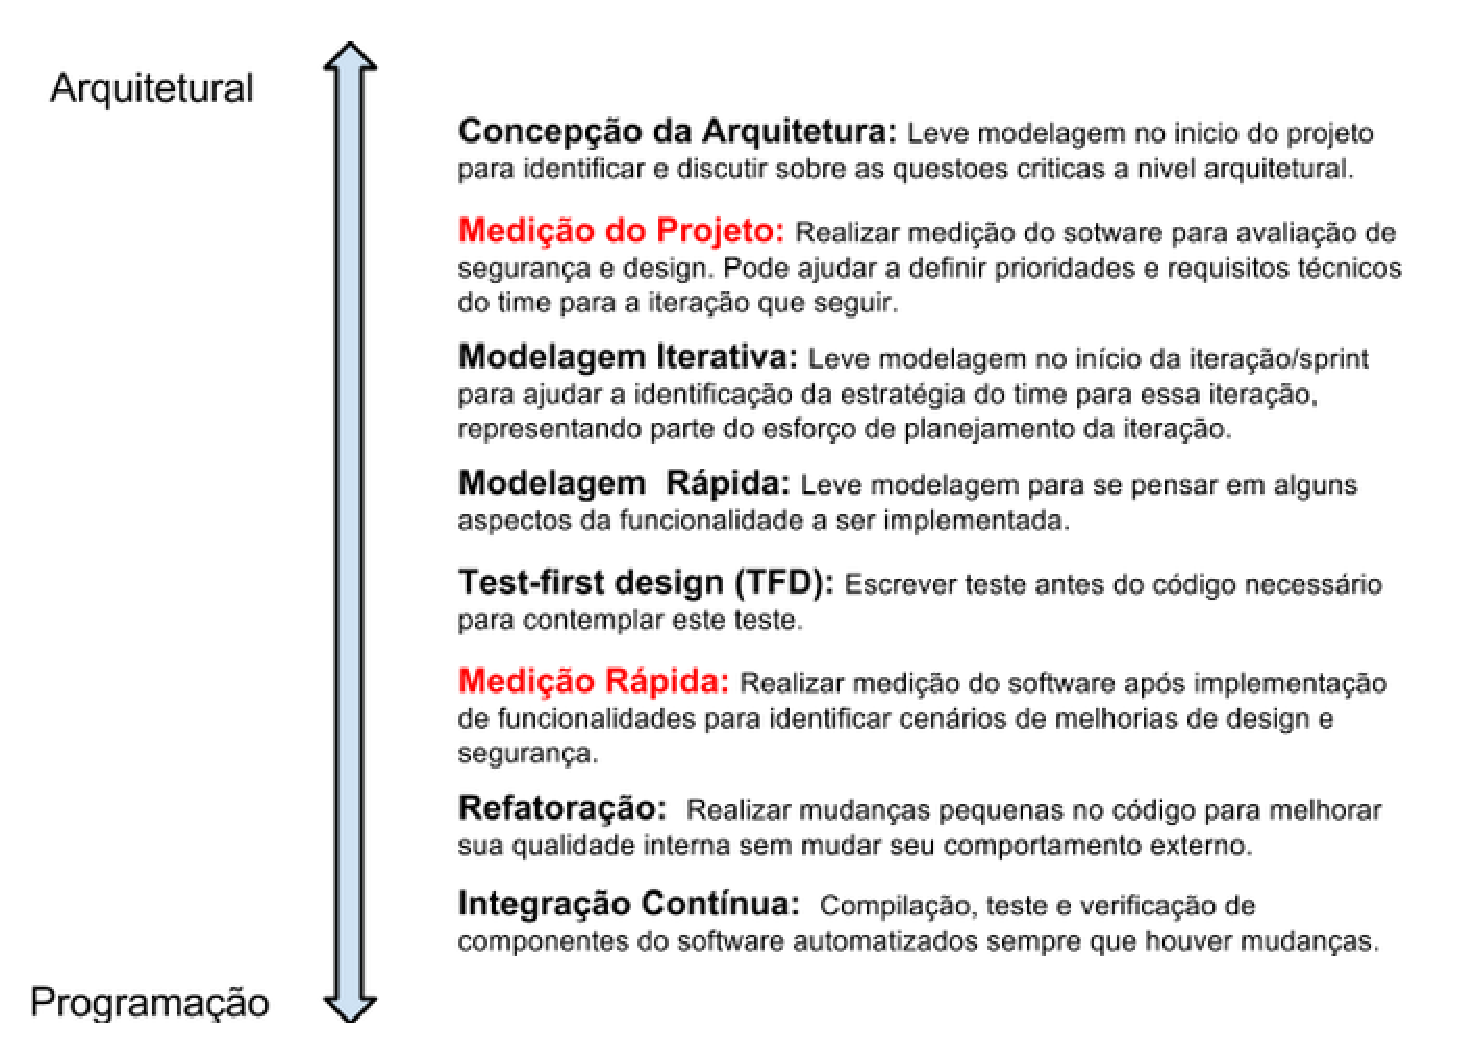
\includegraphics[width=0.8\textwidth]{DesignAgilComMedicao.eps}
\caption{Práticas do Design Ágil Utilizando Métricas de Código-Fonte}
\label{fig:agile-design-metrics}
\end{figure}

%

A prática Medição do Projeto, apresentada na Figura~\ref{fig:agile-design-metrics}, propõe o monitoramento detalhado do código a cada iteração de desenvolvimento. Através desse monitoramento a equipe de desenvolvimento e gestores podem definir e priorizar um conjunto de requisitos técnicos para a próxima iteração que visam atacar os mals cheiros de código identificados, problemas de segurança ou violações do \emph{design}.

%

Na Figura~\ref{fig:agile-design-metrics} ainda propomos a prática Medição Rápida como uma prática a ser utilizada constamente pelo Engenheiro de Software ao evoluir e estender o código. As modificações realizadas durante o desenvolvimento podem gerar incoformidades técnicas indesejadas para o bem estar do código, que por sua vez podem ser identificadas através de métricas. Assim, o Engenheiro de Software teria um melhor suporte para escolher quais são os seus próximos passos, como por exemplo, analisando qual seria a melhor refatoração a ser aplicada. Portanto, a prática de Medição Rápida poderia ser utilizada várias vezes ao longo do desenvolvimento, proporcionando a melhoria contínua do código.

%

Para que as práticas destacadas na Figura~\ref{fig:agile-design-metrics} possam de fato ser utilizadas na melhoria contínua do código, é necessário que os parâmetros de qualidade de um projeto sejam bem definidos e conhecidos pelos membros da equipe técnica. Mais do que isso, é importante que as medições sejam utilizadas para caracterizar o estado do software adequadamente, não baseado somente em interpretações de métricas isoladas, de tal forma que possibilite a tomada de decisão segura.

%

Tendo em vista os benefícios de se utilizar métricas no processo de desenvolvimento de software, buscamos com este trabalho estudar como métricas podem ser utilizadas em projetos de software. Além disso, queremos estudar mecanismos e ferramentas que diminuam as dificuldades inerentes à medição de software, suportando, por exemplo, o trabalho de Engenheiro de Software para tomada de decisões sobre a segurança do código. Neste sentido, no próximo capítulo exploramos dois ambientes diferentes para monitoramento de código-fonte como soluções que podem ser utilzadas por equipes de software.

%

Em busca de mecanismos que facilitem a adoção da medição como prática constante no desenvolvimento de software, no Capítulo \ref{cap-cenarios} é proposto a técnica Cenários de Decisões para utilização de métricas de código-fonte que visa abstrair as métricas para cenários que caracterizem o estado de um código, suportando a tomada de decisões. Ainda neste capítulo fazemos algumas propostas de cenários que utilizam tanto métricas de \emph{design} quanto de segurança para caracterizar estados indesejáveis para a segurança do código.

%

Por fim, o estudo e levantamento de métricas apresentadas no presente capítulo serão a base para a proposta de exemplos de Cenários de Decisões do Capítulo \ref{cap-cenarios}. Além disso, buscamos compreender e relacionar as métricas de \emph{desingn} e vulnerabilidades apresentadas para melhorar o monitoramento e evolução de softwares, dada as motivações apresentadas no Capítulo \ref{cap-metrics}.

%